\documentclass[letterpaper]{article}
\usepackage[T1]{fontenc}
\usepackage{titling, amsmath, amssymb, url, alltt, float, enumitem, graphicx,
multicol, hyperref, listings}
\setlength{\droptitle}{-5em} 
\title{Exploring Dynamic Parallelism in CUDA C with Mandelbrot Sets}
\author{Joseph Zhong
\\ josephz@cs.washington.edu
\\ University of Washington}
\usepackage[top=0.5in, bottom=1in, left=0.5in, right=0.5in]{geometry}
\graphicspath{ {experiments3} {images} }
\setlist{noitemsep}
\setlength{\columnsep}{1cm}

\lstset{
numbers=left,
numberstyle=\tiny,
basicstyle=\footnotesize,
numbersep=8pt,
frame=single,
language=C
}

\hypersetup{
  colorlinks=true,
  linkcolor=blue,
  filecolor=magenta,
  urlcolor=cyan
}

\newcommand{\ind}{\hspace{1cm}} 
\newcommand{\m}[1]{\mathbf{#1}}
\newcommand{\x}{\m{x}}
\newcommand{\bigC}{\mathbf{C}}
\newcommand{\bigX}{\mathbf{X}}
\newcommand{\bigI}{\mathbf{I}}

\begin{document}
\maketitle
\begin{multicols}{2}

  \section{Introduction}

Mandelbrot Sets are a well studied mathematical concept. Mathematically, the set
  of complex numbers is formally defined as the set of complex value $c$ for 
  which the quadratic $z_{n+1} = z_n^2+c$ remains bounded for a large number of 
  iterations $n$ where $z_0 = 0$. We can formally define the mandelbrot set $M$
  as the following for a radius $R$:

  $$M = \{ c \in \mathcal{C} : \exists R \forall n : |z_n| < R  \}$$

Visually, we can create an image of the Mandelbrot set by plotting the complex
  points $c$, assigning membership of the Mandelbrot set $M$. By treating the
  real and imaginary parts of $c$ as our $a$ and $bi$ coordinates in the complex
  plane. In theory, this visualization of the Mandelbrot Set will generate
  infinitely recursing factals at increasing magnification levels throughout the
  shape of the set.

In the context of graphically representing Mandelbrot sets in through computer 
  generated graphics, we can color pixels representing points based on the
  behavior the algorithm used to determine whether a point belongs in the set. A
  common strategy to determine whether a point belongs within the Mandelbrot Set
  is to limit the number of iterations, and assign set membership once the 
  iteration limit has been reached.

Notice that with this strategy, we can notice that complex numbers of real and
  imaginary parts greater than 2 cannot be a part of the set, and thus a common
  cheap and easily implemented strategy is simply to check the complex number's
  parts for exceeding this threshold. While there exist methods which can detect
  set membership quicker such as using Euclidean distance from the origin, for
  simplicity we present this strategy to compute a point's membership.

With this strategy, we can then utilize a color mapping function using the
  iteration limit to assign pixel color values for each point. One simple
  algorithm which utilizes this strategy is known as the Escape Time Algorithm,
  which can compute the per-pixel values of the points within the Set.
  
In this report we compare the performance of the Escape Time Algorithm when 
  implemented naively to calculate the per-pixel value, against an algorithm,
  which takes advantage of the fact that Mandelbrot sets are connected. Thus, by
  only calculating the values of the borders, we can determine whether the inner
  shape can be filled in if the border values are equal. Thus, we can assign
  compute power with finer grain detail, assigning fewer threads to portions of
  the problem, which either complete earlier or uniformly assign pixel value to
  a larger area, while leaving more compute resources for smaller areas of the
  problem which require more time to complete for a smaller area of pixels.

This implementation strategy is also known as Dynamic Parallelism. Parallel
  computation is exploited as our algorithm discovers more parallelizable work
  during runtime, rather than statically dispatching a stringent fixed number of
  parallel compute resources at compile time. In CUDA C specifically, dynamic
  parallelism was introduced in CUDA 5.0 with the Kepler architecture in 2012,
  and is available to devices of Compute Capability of 3.5 or greater. 

We will see that for the initial and conlonical image of a Mandelbrot set that
  we can achieve significant speed up in terms of pixel values computed per 
  second for increasing resolution and iteration limits. Code will be made
  available at \url{https://github.com/joseph-zhong/MandelbrotSets}

  \section{The Escape Time Algorithm}

The Escape Time Algorithm conducts a repeating calculation for each $c$ in our
  plot with a fixed iteration limit. The color assigned for each point is
  determined by a mapping from the number of iterations needed to determine
  membership. The core idea is to quantize our plot into representable pixels
  by coordinates $x$ and $y$, and for each pixel, approximate the likelihood
  that it belongs in the Mandelbrot set. Realize that by definition, that points
  within the set in theory will never ``escape'',  and thus representation
  accuracy is a function of how high the maximum iterations cap is set, along
  with the resolution granularity of the image to subdivide the plot into.
We present the Escape Time Algorithm below.

\noindent\fbox{\parbox{\linewidth}{
\textbf{Algorithm:} Escape Time Algorithm Formulation \\
$x$: Input real value coordinate. \\
$y$: Input imaginary value coordinate. \\
$k$: Input maximum iterations cap. \\

set iterations count to 0. \\
set z value to ($x$, $y$i) \\
\textbf{while} count is less than $k$ or $z^2$ is less than 4: \\
$\text{ }$ $z \leftarrow z^2 + c$ \\
$\text{ }$ increment count \\
return count
}} \\

Recall that the square of a complex number is defined as the following.

$$z^2=(x^2-y^2) + i(2xy)$$

With the output of the escape time algorithm, we then can easily map to a value
  [0,255] to be used as a pixel intensity value. In particular, this value will
  be used to color the corresponding pixel value at $(x, y)$. In languages 
  which do not support complex typing, one must manually compute the real and 
  imaginary operations separately. In our implementation we define a 
  \texttt{complexNum} struct which acts as our complex number. We also define 
  the corresponding complex number operations.
We present our per-pixel kernel implementation below. Note that we abstract the
  Escape Time Algorithm such that it may be used on the host as well.

\begin{lstlisting}
__global__ void cudaNaiveMandelbrotSetsKernel(
    int *d_output, int width, int height, 
    int maxIterations, const float radius, 
    complexNum cMin, complexNum cMax) {

  int x = threadIdx.x + blockIdx.x * blockDim.x;
  int y = threadIdx.y + blockIdx.y * blockDim.y;
  if (x >= width || y >= height) return;

  int value = calculatePixelValue(width, height, 
    maxIterations, cMin, cMax, 
    x, y, radius);
  d_output[y * width + x] = value;
}

__host__ __device__ int calculatePixelValue(
    int width, int height, int maxIterations,
    complexNum cMin, complexNum cMax, 
    int x, int y,  
    const float radius) {
  // Plot bounds. 
  complexNum diff = cMax - cMin;

  // Determine pixel position.
  float xPos = (float) x / width * diff.a;
  float yPos = (float) y / height * diff.bi;

  // Initialize c and z.
  complexNum c = cMin + complexNum(xPos, yPos);
  complexNum z = c;

  int iterations = 0;
  while (iterations < maxIterations 
    && absSquared(z) < radius) {
    z = z * z + c;
    iterations++;
  }
  return iterations;
}
\end{lstlisting}

As modeled from the pseudocode, the iterations is then utilized later in
  assigning colors to each pixel subdividing our plot space. The \texttt{width}
  and \texttt{height} are parameters specifying the resolution size of our
  target image, while \texttt{cMin} and \texttt{cMax} represent the points in
  our complex plane which bound the plot area we wish to work in. Notice that we
  derive our pixel locations by mapping the complex plane into the domain of the
  \texttt{height} and \texttt{width}, and scale the points with the relative
  positions of \texttt{x} and \texttt{y}.
With this implementation, we can easily launch a kernel which assigns a thread
  to each pixel, and simply calculate the per-pixel value using the Escape Time
  Algorithm.
We present our per-pixel kernel launch below.

\begin{lstlisting}
__host__ void cudaNaiveMandelbrotSets(
    int height, int width, 
    int maxIterations, const float radius, 
    const complexNum cMin, const complexNum cMax, 
    const char *filename) {
  // Host input setup: image.
  const int OUTPUT_SIZE = 
    sizeof(int) * height * width;
  int *h_output = (int*) malloc(OUTPUT_SIZE);

  // Device output setup: image.
  int *d_output;
  cudaCheck(cudaMalloc(&d_output, OUTPUT_SIZE));

  // Kernel Size.
  dim3 gridSize(ceil(width / TILE_WIDTH), 
                ceil(height / TILE_WIDTH), 1); 
  dim3 blockSize(TILE_WIDTH, TILE_WIDTH, 1); 

  // Begin timer.
  clock_t start = clock();

  // Launch Kernel.
  cudaNaiveMandelbrotSetsKernel
      <<<gridSize, blockSize>>>(
      d_output, width, height, maxIterations, 
      radius, cMin, cMax);

  // Synchronize across threads once completed.
  cudaCheck(cudaThreadSynchronize());

  // Stop timer.
  endClock(start);

  if (filename != NULL) {
    // Copy output.
    cudaCheck(cudaMemcpy(h_output, d_output, 
              OUTPUT_SIZE, 
              cudaMemcpyDeviceToHost));    

    // Write to output.
    saveImage(filename, h_output, width, height, 
              maxIterations);
  }   

  // Free output.
  cudaFree(d_output);
  free(h_output);
}
\end{lstlisting}

While this kernel formulation strategy greatly takes advantage of parallelizable
  work, assigning each available thread to compute the membership of each
  data-independent pixel, the fact that the Mandelbrot set is connected is
  overlooked. Within the mandelbrot set, there are large plots of area which the
  neighboring pixels could all be immediately assigned membership, saving
  significant compute time and device resources. In particular, here the
  algorithm spends the most resources computing the points within the mandelbrot
  set for large maximum iteration caps. 
However, when we utilize the fact that the Mandelbrot set is connected, we can 
  greatly reduce compute resources required to assign membership, and instead, 
  allow additional resources to compute membership along the fractal boundary, 
  where iterations will be still high, but of a unique recursively repeating 
  pattern of fine grained detail.
Let us introduce the Border-Tracing Algorithm and modify our above
  implementation to utilize dynamic parallelism to achieve finer granularity
  computation for the above motivated scenario.

  \section{The Border-Tracing Algorithm}

The Border-Tracing Algorithm deviates from the original per-pixel kernel method
  by instead, assigning patches of the plot to each thread, where the goal of
  each parallel thread determines the membership of the entire patch if
  possible. The algorithm takes advantage of the property that Mandelbrot Sets
  are connected. Thus, in theory, if an arbitrary closed polygon has borders of
  uniform values, then we can determine that the pixels within also share the
  value. 
In practice, this algorithm works under the assumption of fine enough grain
  resolution to capture the subtle fractal pattern at the fringe of the
  Mandelbrot set. Additionally, rather than computing the borders of arbitrary
  polygons, rectangles are used instead as the rectangle borders are easier to
  represent. Additionally, with rectangles, we can recursively repeat the
  algorithm to operate on sub-rectangles.
Thus, the core idea is to utilize the Escape Time Algorithm only on the border
  of our selected rectangle, filling the internal pixels with the uniform
  border's value if possible. Otherwise we split the rectangle and recurse.
One additional optimization to realize is that at some cutoff, our
  sub-rectangles will eventually become small enough such that the overhead
  involved with checking the border values and continuously recursing will
  outweigh simply running our Escape Time Algorithm kernel.
We present the Border-Tracing Algorithm below. 

\noindent\fbox{\parbox{\linewidth}{
\textbf{Algorithm:} Border-Tracing Algorithm Formulation \\
$x$: Input real value coordinate of our rectangle. \\
$y$: Input imaginary value coordinate of our rectangle. \\
$w$: Input width of our rectangle. \\
$h$: Input height of our rectangle. \\
$threshold$: Input cut off threshold for small rectangles. \\

border = pixels[$(x,y)$:$(x+w,y)$] \\
$\text{ }$ + pixels[$(x+w,y)$:$(x+w,y+h)$] \\
$\text{ }$ + pixels[$(x,y)$:$(x,y+h)$] \\
$\text{ }$ + pixels[$(x,y+h)$:$(x+w,y+h)$] \\
\textbf{for} every pixel along the border: \\
$\text{ }$ Compute the value with the Escape Time Algorithm. \\
\textbf{if} every pixel value along the border is the same: \\
$\text{ }$ Fill every pixel within the border. \\
\textbf{else if} $w * h < threshold$:  \\
$\text{ }$ Calculate every pixel within the border. \\
\textbf{else}:  \\
$\text{ }$ Split our rectangle into sub-rectangles and recurse.
}} \\

With this implementation, implementation complexity has increased over the
  per-pixel Escape Time Algorithm, and thus has produced the opportunity for
  finer-grain implementation optimization. Notice that through the introduction
  of Dynamic Parallelism in CUDA, we can implement the 
  \texttt{Fill every pixel...} block as a dynamically parallel kernel. Through 
  Dynamic Parallelism, we can reuse our previous Escape Time Algorithm kernel
  for the \texttt{Calculate every pixel within...} block.
Recall that the in our previous implementation using the per-pixel Escape Time
  Algorithm kernel, that every pixel was assumed to be entirely independent.
  Notice that this pseudocode takes into account computational intensity as a
  patch area over our plot. Ideally we should only be computing independent 
  per-pixel values near the fringe of the Mandelbrot set fractal, which in
  general would be at miniscule scale relative to the overall image size and
  thus should receive per-pixel granular computation.
We present our implementation of the kernels below.

Below is the Border-Tracing Kernel.

\begin{lstlisting}
__global__ void cudaDPMandelbrotSetsKernel(
    int height, int width, int maxIterations,
    complexNum cMin, complexNum cMax, 
    int x0, int y0, int size, int depth, 
    const float radius, int *d_output) {
  x0 += size * blockIdx.x;
  y0 += size * blockIdx.y;

  int borderVal = calculateBorder(width, height, 
                  maxIterations, cMin, cMax, 
                  x0, y0, size, radius); 

  if(threadIdx.x == 0 && threadIdx.y == 0) {
    if (borderVal != -1) {
      dim3 fillBlockSize(BLOCK_SIZE, 
         DIVIDE_FACTOR);
      dim3 fillGridSize(divup(size, BLOCK_SIZE), 
         divup(size, DIVIDE_FACTOR));
      fillKernel<<<fillGridSize, fillBlockSize>>>(
  width, x0, y0, size, borderVal, d_output);
    }
    else if (depth + 1 < MAX_DEPTH 
  && size / DIVIDE_FACTOR > MIN_SIZE) {
      dim3 recurseGridSize(DIVIDE_FACTOR, 
         DIVIDE_FACTOR);
      dim3 recurseBlockSize(blockDim.x, 
        blockDim.y);
      cudaDPMandelbrotSetsKernel
        <<<recurseGridSize, recurseBlockSize>>>(
          height, width, maxIterations, 
          cMin, cMax, x0, y0, 
          size / DIVIDE_FACTOR, 
          depth + 1, radius, d_output); 
    }
    else {
      dim3 pixelGridSize(divup(size, BLOCK_SIZE), 
         divup(size, DIVIDE_FACTOR));
      dim3 pixelBlockSize(BLOCK_SIZE, 
        DIVIDE_FACTOR);
      pixelKernel
  <<<pixelGridSize, pixelBlockSize>>>(
    width, height, maxIterations,
    cMin, cMax, x0, y0, size, radius, d_output);
    }
  }
}
\end{lstlisting}

Below is the \texttt{calculateBorder} implementation. 

The Escape Time Algorithm is utilized to load pixel values on the border into
  shared memory, where a parallel reduction is used to reduce the border values
  into a common value if it exists, or a failure flag otherwise. 

\begin{lstlisting}
__device__ int calculateBorder(int width, 
  int height, int maxIterations, complexNum cMin, 
  complexNum cMax, int x0, int y0, int size, 
  const float radius) {

  int tIdx = threadIdx.y * blockDim.x 
      + threadIdx.x;
  int blockSize = blockDim.x * blockDim.y;

  // Set default to just above cap.
  int value = maxIterations + 1;

  // Determine common value if possible.
  for (int pixel = tIdx; pixel < size; 
			pixel += blockSize) {
    for (int boundary = 0; boundary < 4; 
				boundary++) {
      int x = boundary % 2 != 0 ? x0 + pixel : 
          (boundary == 0 ? x0 + size - 1 : x0); 
      int y = boundary % 2 == 0 ? y0 + pixel : 
          (boundary == 1 ? y0 + size - 1 : y0);
      value = commonValue(value, 
        calculatePixelValue(width, height, 
          maxIterations, cMin, cMax, x, y, radius), 
          maxIterations);
    }
  }

  // Load values into shared memory.
  __shared__ int s_output[BLOCK_SIZE 
      * DIVIDE_FACTOR];
  int numThreads = min(size, BLOCK_SIZE 
      * DIVIDE_FACTOR);
  if (tIdx < numThreads) {
    s_output[tIdx] = value;
  }
  __syncthreads();

  // Parallel Reduction to common value.
  for(; numThreads > 1; numThreads /= 2) {
    if (tIdx < numThreads / 2) {
      s_output[tIdx] = commonValue(s_output[tIdx], 
            s_output[tIdx + numThreads / 2], 
            maxIterations);
    }
    __syncthreads();
  }
  // Reduced output.
  return s_output[0];
}
\end{lstlisting}

Below is the \texttt{fillKernel} implementation. 
Notice its stark similarity to the original per-pixel implementation.

\begin{lstlisting}
__global__ void pixelKernel(int width, int height, 
    int maxIterations, complexNum cMin, 
    complexNum cMax, int x0, int y0, int size, 
    const float radius, int *d_output) {
  int x = threadIdx.x + blockDim.x * blockIdx.x;
  int y = threadIdx.y + blockDim.y * blockIdx.y;

  if (x < size && y < size) {
    x += x0;
    y += y0;
    d_output[y * width + x] = calculatePixelValue(
      width, height, maxIterations, cMin, cMax, x, 
      y, radius);
  }
}
\end{lstlisting}

Below is the \texttt{pixelKernel} implementation.
Notice its stark similarity to the original per-pixel implementation.

\begin{lstlisting}
__global__ void fillKernel(int width, int x0, 
    int y0, int size, int value, int *d_output) {
  int x = threadIdx.x + blockIdx.x * blockDim.x;
  int y = threadIdx.y + blockIdx.y * blockDim.y;

  if (x < size && y < size) {
    x += x0;
    y += y0;
    d_output[y * width + x] = value;
  }
}
\end{lstlisting}

One major difference however, is to realize that the above two kernels were
  launched \textbf{from the device} with parallelizable work discovered at 
  runtime, rather than being prepared and run once after compile time! This is
  the core of Dynamic Parallelism: the capacity to \textbf{allocate device
  memory and parallel tasks from children of the host}.
In general, we can see that the kernels implementing the Border-Tracing
  algorithm outperform the kernels naively utilizing the Escape Time algorithm.

  \section{Experiment Design}

We specifically chose not to analyze GFLOPs as we deemed that it was a
  deceptive metric in determining performance. While in measuring quality of
  hardware, it serves to demonstrate the speed and robustness of an
  architecture, in terms of algorithm and software design, the goal is not
  necessarily measured in number of operations. Rather we care about the number
  of outputs per cost. 
While GFLOPs and outputs per cost are heavily correlated, in this specific case
  study, note that the Border-Tracing algorithm optimizes the previous algorithm
  by entirely skipping operations, while potentially significantly increasing
  outputs per cost metric. To maintain this correlation, we choose our cost
  metric as time as it is heavily correlated with expensive computation in terms
  of energy, and is a useful metric in general, barring consistency within
  environments.
To address this consistency issue, we choose then to run all experiments on the
  same machine with a NVIDIA GeForce GTX 1060 graphics card with 6GB of GDDR5
  VRAM, 1280 CUDA Cores, a Graphics Clock rated 1.506GHz and a Processor Clock 
  rated 1.708GHz. It was important to have a graphics with a high memory
  configuration as we suspected that at inputs of low memory requirement would
  finish too quickly to provide significant results, in particular with respect
  to outputs per cost. 
More importantly, devices with Compute Capability of at least 3.5 are required to
  utilize Dynamic Parallelism, which has Compute Capability of 6.1.

The primary experiments we analyze between the algorithms are as follow:

\begin{itemize}
  \item Million Pixels per second output rate.
  \item Total Kernel Running Time. 
  \item The impact of increased iteration cap.
  \item The impact of increased output resolution.
\end{itemize}

To measure the above experiments, we set a baseline iteration cap at 256, and a
  baseline resolution starting at 2048x2048. We then increase the two parameters 
  by a factor of 25\% a total of 12 times, running 10 trials to average, and
  take the min and max running times in seconds. 
Each of the individual MP/s and Total Kernel Running Time experiments were ran
  by setting the baseline variable of either iteration cap or resolution, and
  varying the other variable.  
We set a maximum resolution of 23150x23150 pixels, which is a bit before the
  point at which we empirically began to run out of memory on our GPU.
All of our experiments were run on the initial Mandelbrot Set coordinates, at
  (-1.5, -1) to (0.5, 1).

  \section{Results}

The below graphs were all generated through our \url{run.py} script using
  \texttt{matplotlib} and \texttt{subprocess}. 

\textbf{Note:} While included in our code is functionality to generate results
  using the host hardware, we have not included experiments as we concluded from
  our short experiments that sequential implementations were simply entirely too
  slow to compare with either of the data parallel implementations.

We see from Figure \ref{fig:mppsIter} that our Border-Tracing kernel
  outperforms the naive implementation across each iteration cap by a factor of
  about 200\%. Interestingly, as the iteration cap increases, the variance
  amongst the trials of the Border-Tracing kernel decreases, with nearly no 
  variance between the minimum and maximum trials towards the latter half of the 
  experiment. Also interesting to note that the naive kernel consistently has
  nearly no variance throughout each of the trials. 
Overall from the logarithmic behavior of this plot perhaps indicates that as the
  iteration cap increases, that benefit of parallelism dwindles as the problem
  becomes increasingly compute bound.  

In Figure \ref{fig:mppsRes}, we can very obviously that the Border-Tracing
  kernel by far outperforms the naive implementation at every resolution.
  Interesting to see is how the naive solution nearly behaves as a step
  function, where at around 800x800, the efficiency of the kernel suddenly jumps
  up to nearly 1000 MPix/s from the previous base of around 800 MPix/s.
The trend continues from Figure \ref{fig:mppsIter}, where the variance between
  the two implementations significantly differs, where the naive implementation
  is very stable while here the variance of the Border-Tracing kernel has
  increased significantly throughout the experiment.

\begin{figure}[H]
  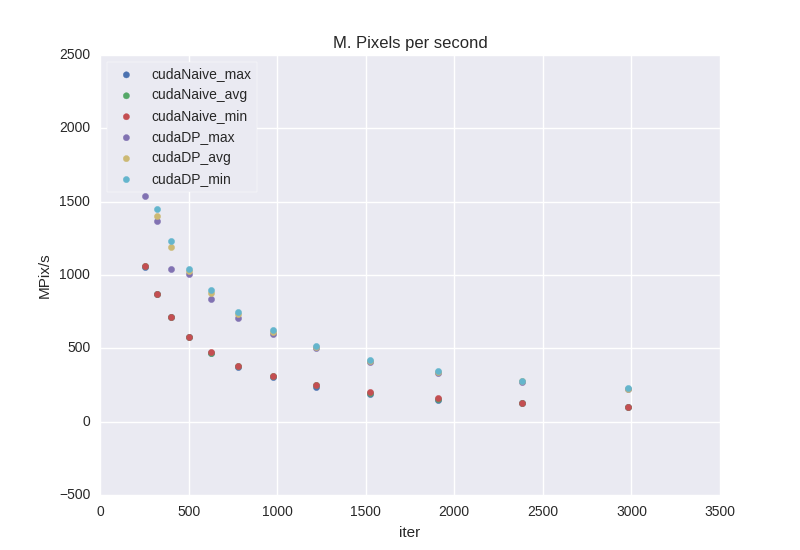
\includegraphics[width=\linewidth]{experiments3/mpps_graph_exp_iter.png}
  \caption{Megapixels per second, varying iteration cap.}
  \label{fig:mppsIter}
\end{figure}

\begin{figure}[H]
  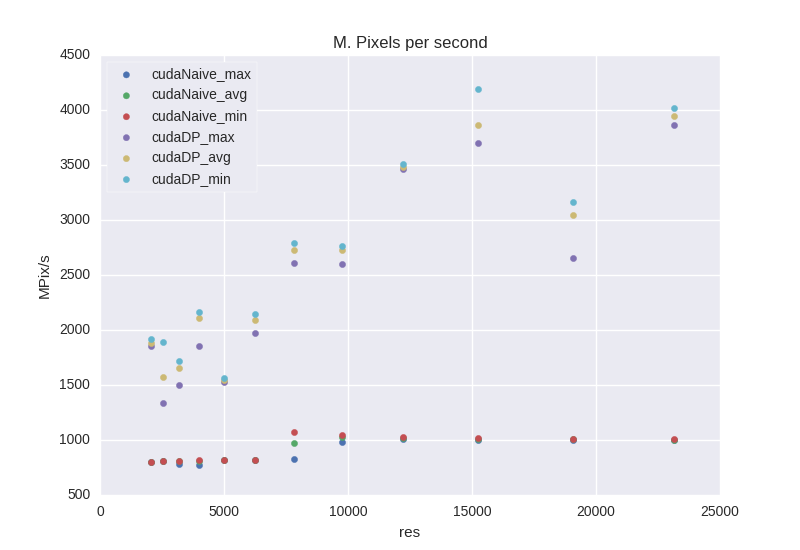
\includegraphics[width=\linewidth]{experiments3/mpps_graph_exp_res.png}
  \caption{Megapixels per second, varying image resolution.}
  \label{fig:mppsRes}
\end{figure}



Additionally, it is interesting to think about the behavior of the averages.
  Through 15Kx15K resolution, the efficiency of the Border-Tracing kernel seems
  to monotonically increase. This is perhaps best explained through the fact
  that as resolution is increased, the number of pixels within the set grow
  exponentially, but the method of the Border-Tracing Algorithm is able to keep
  up with the growth as the number of pixels which need per-pixel granularity
  computation is not growing as quickly. 
However, more interesting is the sudden drop in performance at around 19Kx19K
  resolution. Perhaps if we had a graphics card of greater memory capacity, we
  would be able to see that past 15K resolution, that the behav,ior of the curve
  is in fact logrithmic, and that we would see little to no growth in
  performance beyond 15K. 
It is also that at around 19K resolution, that we have hit a pathological case
  in which each subsequent subdivision in the rectangles continuously has border
  values which are not uniform until the subdivisions are very small, causing
  the sudden drop in performance.

\begin{figure}[H]
  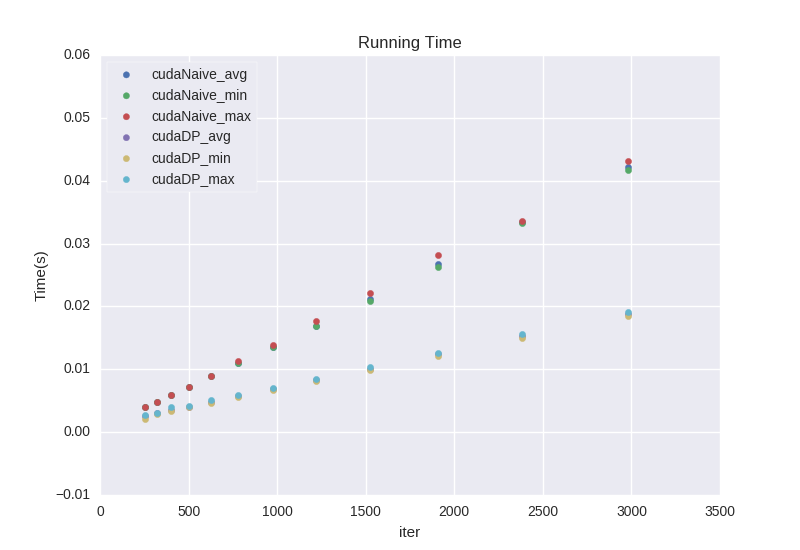
\includegraphics[width=\linewidth]{experiments3/running_time_graph_exp_iter.png}
  \caption{Kernel running time, varying iteration cap.}
  \label{fig:rtIter}
\end{figure}

\begin{figure}[H]
  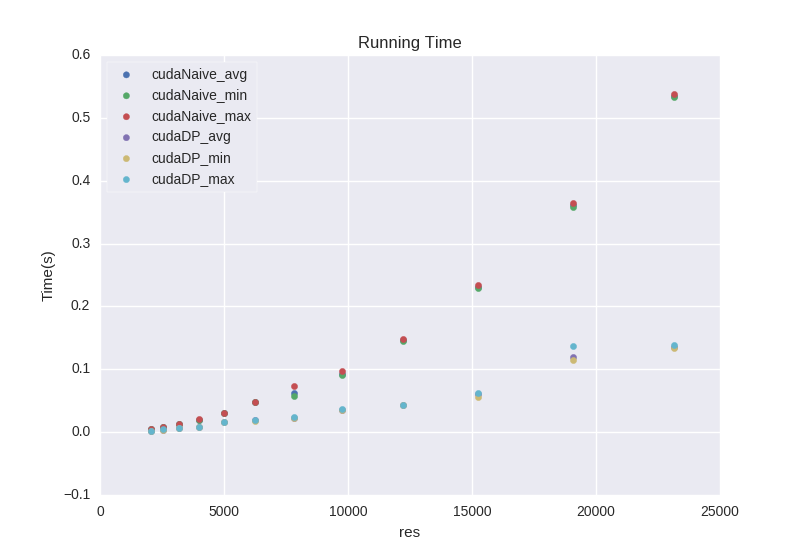
\includegraphics[width=\linewidth]{experiments3/running_time_graph_exp_res.png}
  \caption{Kernel running time, varying image resolution.}
  \label{fig:rtRes}
\end{figure}

With the Running time against iteration cap shown in Figure \ref{fig:rtIter}, it
  is obvious to see the performance increase which the Border-Tracing kernel has
  over the naive implementation, again consistently running in half the time in
  seconds. Unlike the previous experiments (See Figures \ref{fig:mppsRes} and
  \ref{fig:mppsIter}), it seems as though the variance for naive implementation
  of the Escape Time Algorithm is ever so slightly greater than its counterpart.
However the previous two experiments in MPix/s would indicate that the
  Border-Tracing Algorithm is more volatile, depending on dynamically
  discoverable parallel work, and thus leading to more variable running times
  depending on which portions of the plot are computed on. 

In that view, it makes sense that this experiment had particularly low variance,
  as we fixed the baseline resolution to 2048x2048 while varying the iteration
  cap. It seems intuitive that a linear increase in difficulty leads to a linear
  increase in compute time, as the actual size and number of compute resources
  dispatched remains constant throughout the experiment. 

In Figure \ref{fig:rtRes}, we see once again that the running time over
  increasing resolution leads to very low varying results, just as in the other
  Running time experiment (See Figure \ref{fig:rtIter}). We can see that at very
  small problems, the difference between the two kernels are nearly
  indistinguishable. Although both curves seem to follow an exponentially
  growing behavior, the naive Escape Time Algorithm kernel grows vastly faster
  than the Border-Tracing counterpart. At 23K resolution, the Border-Tracing
  counterpart nearly has 20\% the running time of the naive kernel.
  Interestingly, we see here that at 19K the Border-Tracing kernel perhaps took
  an unusual amount of time, resulting in the previously seen sudden drops in
  performance efficiency (See Figure \ref{fig:mppsRes}).  

  \section{Conclusions and Future Work}

In this report, we present data parallel algorithms for Mandelbrot Set image
  computation, where the methods we have presented can be utilized as
  subroutines in computer graphics applications. Additionally, we have released
  code which can be helpful for running timing and kernel performance
  experiments for future use. The core idea behind this report was to explore
  the potential power of Dynamic Parallelism. 
Given the significant theoretical and mathematical backing behind the generation 
  of fractals and Mandelbrot sets, there is substantial future work which lies 
  ahead, including the analysis of generalized fractal generation algorithms
  such as Julia Sets, and variations of Mandelbrot Sets. 
Thanks to significant development in the CUDA programming model in recent years,
  we can perhaps see increases in algorithm design which can better utilize the
  capabilities of increasingly powerful and flexible hardware. 

\end{multicols}



\end{document}





